\section{Réflexions sur les données}

Nous avons créé différentes structures de données qui seront transmises par les composants du système et qui contient toutes les informations que nous en avons besoin. \\

\begin{itemize}
\item \textbf{SensorData} – cette structure contient les informations transmises par le capteur (identifiant du capteur et la donnée transmise).
\item \textbf{SensorConfig} –  structure utile pour paramétrer les capteurs.
\item \textbf{DevicePosition} – contient les informations de position du dispositif.
\item \textbf{DevicePower} – contient les informations de l’autonomie énergétique du dispositif.
\item \textbf{InfoData} – structure enregistrée par le serveur pour la traçabilité.
\end{itemize}

Les données seront transmises entre le système embarqué, les capteurs et le serveur central, comme dans le schéma suivant : \\

    \begin{figure}[!h]
    \begin{center}
    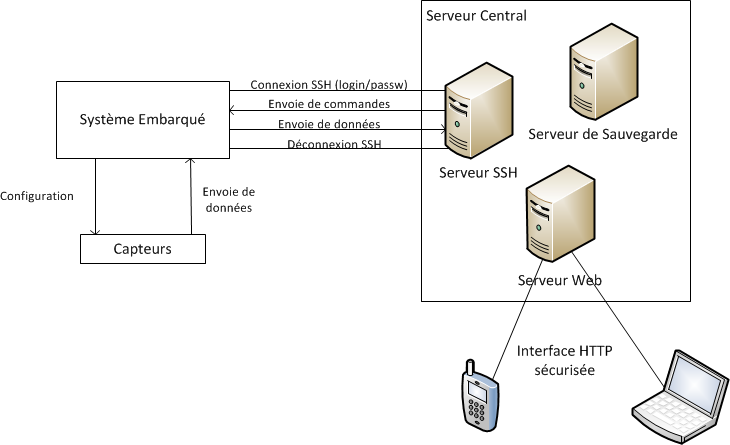
\includegraphics[width=4cm]{\PIXPATH/donnees1}
    \caption{}
    \end{center}
    \end{figure}

Les détails des structures de données peuvent être vus à  l’annexe A 1 : Représentation informatique des objets.
Les commandes possibles utilisées par le Serveur Central sont : \\

\begin{itemize}
\item \textbf{GetData} – Demande les données de tous les capteurs de la station concerné. Reçois comme réponse une liste non chainé de la structure InfoData  - InfoDataList.
\item \textbf{GetPosition} – Demande la position exacte de la station concerné.
\item \textbf{GetPower} – Demande l’autonomie d’Energie de la station.
\item \textbf{ConfigData <SensorId> <min> <max>} - Configure le seuil minimum et maximum critique du type de donnée concerné du capteur. Le type de données peut être, par exemple,  la température, la hauteur d’un réservoir, etc.
\end{itemize}

